\documentclass[11pt]{article}

\usepackage{color}
\usepackage{caption}
\usepackage{amsmath}
\usepackage{amsthm}
\usepackage{amsfonts} 
\usepackage{amssymb}
\usepackage{multirow}
\usepackage[pdftex]{graphicx}
\usepackage{epsfig}
\usepackage{latexsym}
\usepackage{enumerate}
\usepackage{tabularx}
\usepackage{booktabs}
\usepackage{fullpage}
\usepackage{algorithm}
\usepackage{centernot}
\usepackage[noend]{algpseudocode}

\newtheorem{thm}{Theorem}
\newtheorem{problem}[thm]{Problem}
\newenvironment{claim}[1]{\par\noindent\textit{Claim:}\space#1}{}

\newcommand{\R}{\mathbb{R} }
\newcommand{\Q}{\mathbb{Q} }
\newcommand{\Z}{\mathbb{Z} }
\newcommand{\N}{\mathbb{N} }
\newcommand{\C}{\mathbb{C} }
\newcommand{\Prob}[1]{ \mathbb{P} \left[ #1 \right] }
\newcommand{\Given}{\middle|}
\newcommand{\overbar}[1]{\mkern 1.5mu\overline{\mkern-1.5mu#1\mkern-1.5mu}\mkern 1.5mu}

\begin{document}

\title{Visualizing Hillary Clinton's Emails}

\author{
  Yihe Chen \\
  \texttt{yc3076}
  \and 
  Palmer Lao \\
  \texttt{pol2105}
  \and
  Daitong Li \\
  \texttt{dl2991}
  \and
  Ziyue Shuai \\
  \texttt{zs2285}
  \and
  Eric Zhang \\ 
  \texttt{ez2232}
}

\date{\today}
\maketitle
\section{Social Network Analysis}
Instead of exploring the e-mail content, we are also interested in examining the interaction and connections through the Hillary Clinton's e-mail exchange. We focus on the receivers and senders of all the e-mails and build a social network based on the correspondence using Social Network Analysis (SNA) techniques from the study of Sociology. In subsection \ref{sna_data}, we will walk through the data configuration catered to the process of SNA. The visualization of the network will be presented in Subsection \ref{sna_nw}. Following Subsection \ref{sna_nw}, we dive into the properties of the network using some common metrics in SNA and further explore the subgroups in the network to detect potential communities.
\subsection{Data Configuration}\label{sna_data}
Wikipedia summarizes that SNA  is the process of investigating social structures\cite{wiki_sna}. The structure consists of two parts, individuals and interactions, graphically characterized as nodes and edges in the network. And the data sets for our SNA are set up in such format (see Figure \ref{fig:node_file} and \ref{fig:edge_file} for snapshots of the data sets).
\begin{figure}[ht]
\caption{Nodes file snapshot}
\label{fig:node_file}
\centering
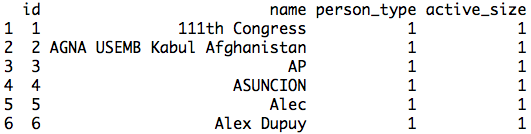
\includegraphics[width=.68\textwidth]{report_node_file}

\caption{Edges file snapshot}
\label{fig:edge_file}
\centering
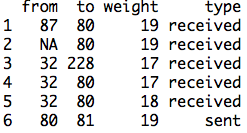
\includegraphics[width=.35\textwidth]{report_edge_file}
\end{figure}

In the parlance of SNA, the nodes represent all $513$ individuals involved in Hillary Clinton's e-mails based on the \verb+``Persons.csv''+ file from Kaggle. Each person has a distinctive Person ID, and  some of the intuitive key players and their IDs are the following:
\begin{table}[ht]
\caption{Key individual by intuition}
\label{tab:int_key}
\centering
\begin{verbatim}
		#    id            name
		#    80 Hillary Clinton
		#    81 Huma Abedin
		#    87 Jake Sullivan
\end{verbatim}
\end{table}

We also assign a type and a weight to each node, which are the \verb+person_type+ and \verb+active_size+ variables in Figure \ref{fig:node_file}. The node type captures the characteristic of the person and is set up as below (see Table \ref{tab:node_type} for a simple overview for \verb+person_type+ by counts):
\begin{itemize}
\item \verb+person_type =  3+, node \verb+name+ is Hillary Clinton;
\item  \verb+person_type =  2+, node \verb+name+ contains ``\verb+@state+''. \\That is, the person name is an governmental email address;
\item \verb+person_type =  1+, all the others,\\
 including people with full names, fragmented name, or unidentifiable aliaises.
\end{itemize}

\begin{table}[ht]
\caption{Overview of Node Type}
\label{tab:node_type}
\centering
\begin{tabular}{l | r r r}
\verb+person_type+ & 1 & 2&3\\ \hline 
count & 355 & 157 &1
\end{tabular}
\end{table}

The weight of each node measures the level of activeness of each individual. The weight for Person $i$ is calculated as 

\begin{equation} 
\verb+active_size+ = \mbox{frequency Person $i$ as Sender} +  \mbox{frequency Person $i$ as Receiver}
\end{equation}
\verb+active_size+ has to be at least $1$ to appear in Hillary's e-mails. And a brief summary of the Node Size is shown in Table \ref{tab:node_size}
\begin{table}[ht]
\caption{Overview of Node Size}
\label{tab:node_size}
\centering
\begin{tabular}{llllll}
Min. &1st Qu. & Median&    Mean& 3rd Qu.  &  Max. \\ \hline
   1.00 &   1.00  &  1.00&   33.32 &   2.00 &7580.00 
 \end{tabular}
\end{table} 
 
From Table \ref{tab:node_size}, we see the distribution of \verb+active_size+ is highly skewed, as the quantiles are extremely small and close to each other, while the mean and maximum are extremely large. And we can in fact identify some key individuals by the node size extrema alone - four people with \verb+active_size+ $> 1000$ are the three people in Table \ref{tab:int_key} and Person 32: \verb+Cheryl Mills+.

To better describe the interaction, we use directed graph to depict the network based on the \verb+``Receivers.csv''+ and \verb+``Emails.csv''+ from Kaggle. Hence, we set up variables \verb+from+ and \verb+to+ in the Edges file in Figure \ref{fig:edge_file} to capture direction of the email flow. The Edges file keeps track of a total of $9306$ pairs of one-to-one interaction in $7945$ e-mails. The discrepancy is caused by e-mails with multiple receivers (Hillary is one of the receivers or Hillary sent an e-mail to multiple people).

The edges also have two attributes: \verb+weight+ and \verb+type+. The edge type is labeled as below  
\begin{itemize}
\item \verb+type+ = ``received'', if the corresponding e-mail was received by Hillary (and other people);
\item \verb+type+ = ``sent'', if the corresponding e-mail was sent by Hillary (to one person or more);
\item \verb+type+ = ``other', if the Sender is marked as ``NA'' in the original Kaggle data file.
\end{itemize}

Table \ref{tab:edge_type} shows that Hillary Clinton's inbox had more incoming (``received'') e-mails than outgoing ones. A side-by-side network graphs by edge type  will be supplied in Subsection \ref{sna_nw} in order to visually compare these two types of interaction.  
\begin{table}[ht]
\caption{Overview of Edge Type}
\label{tab:edge_type}
\centering
\begin{tabular}{l | r r r}
\verb+type+ & other & received & sent\\ \hline 
count & 13 & 6549 &2744
\end{tabular}
\end{table}

The edge weight is also devised to identify different interaction pattern. The idea is to accumulate weights as the frequency of e-mail exchange between two individuals increases. But we also want to reward exclusivity of two individuals, so we lower the weight if the corresponding e-mails between two individuals involves other people. Therefore, we came up with the following weighting scheme for edge $j$ where $j \in \{1,2 , \cdots, 9306\}$.\begin{enumerate}
\item Start with initial weight, \verb+weight+$_j = 20$;
\item Find the corresponding e-mail ID for edge $j$, ID$_j = k$  where $k \in \{1, 2, \cdots, 7945\}$;
\item Count the number of Receivers for e-mail $k$, $N_{kr}$ and the number of people Cc'ed, $N_{kc}$;
\item Final weight for edge $j$ is calculated as
\begin{equation}
\verb+weight+_j = 20 - N_{kc} - N_{kr}
\end{equation}
\end{enumerate}
Before building the network, we collapse all the edges between the same two nodes by summing their weights and ended up with $739$ distinct directional edges\footnote{``Directional'' in the sense that edges $A \rightarrow B$ and $B \rightarrow A$ were not collapsed. }.
\begin{table}[ht]
\caption{Overview of Edge Size}
\label{tab:edge_size}
\centering
\begin{tabular}{llllll}
Min. &1st Qu. & Median&    Mean& 3rd Qu.  &  Max. \\ \hline
   7.0    &17.0  &  18.0 &  225.8   & 49.5&25640.0 
 \end{tabular}
\end{table} 

Since this is a one-person-centered network, summary statistics of edge weight in Table \ref{tab:edge_size} also have an extremely large maximum comparing to the mean and 3rd quartile. In the upcoming subsection, we make use of the 1st quartile as the cut-off value and cull the edges to make the graph more informative.

\subsection{Network Visualization} \label{sna_nw}
In this subsection, we will present varied ways to visualize the network and some techniques to improve the visualization by using the attributes of the edges and nodes.

\begin{figure}[ht]
\centering
\caption{Improved Network after Deleting Low-weight Edges}
\label{fig:improvednw}
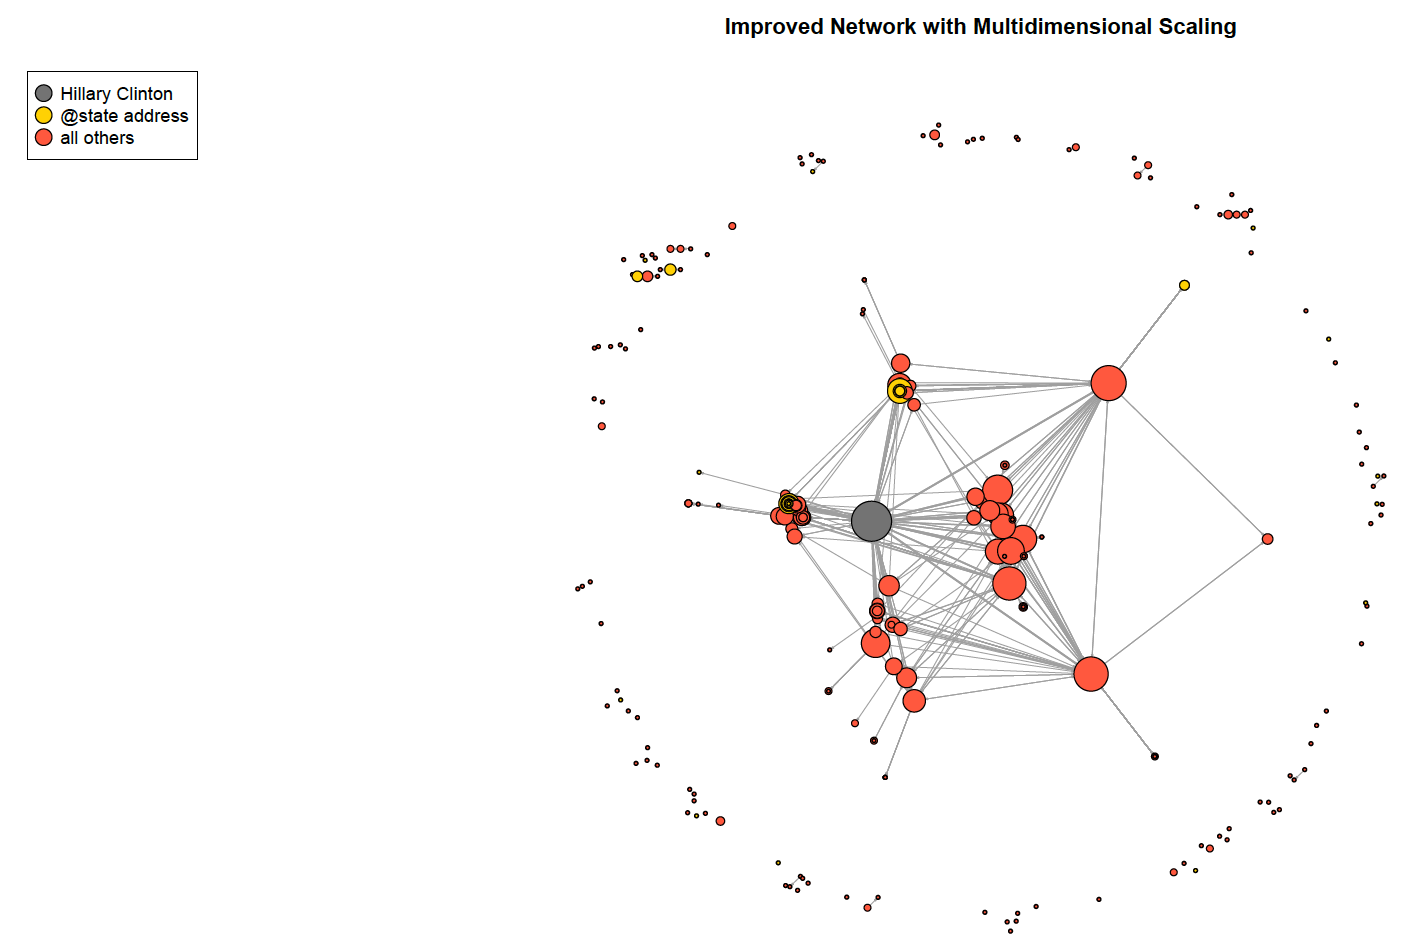
\includegraphics[width = 1\textwidth]{report_dms_layout}
\end{figure}

One key factor for effective visualization of a network is the graph layout. We have compared $15$ different types of layout and decided to display our network with the Multidimensional Scale layout. The algorithm behind each layout scheme is beyond the scope of our discussion in this report, but we do invite the readers to see Appendix \ref{App:AppendixA} Figure \fbox{empty ref?}  and compare all $15$ layouts we have tested.

The natural choice of color and size for nodes is based on the values of variables ``\verb+person_type+'' and ``\verb+active_size+''. See the legend in Figure \ref{fig:improvednw} to understand the colorcode. Table \ref{tab:node_size} in the previous subsection suggests the distribution of node size is highly skewed, hence we need to rescale it to make it i) more reasonable as iGraph object input as the default is $15$ and ii) have less variance. Inspired by the variance-stablizing transformation, we devised the following rescaling scheme in Equation (\ref{eqt:rescale}). The side-by-side histograms in Figure \ref{fig:rescalenode} demonstrates that this rescaling scheme is effective. The similary log-transform rescaling was also applied to the edge weight, which is also highly skewed.
\begin{equation}
\label{eqt:rescale}
\verb+rescaled active_size+ = \log \verb+active_size+ + 1
\end{equation}
\begin{figure}[ht]
\caption{Rescaling of Node Size}
\label{fig:rescalenode}
\centering
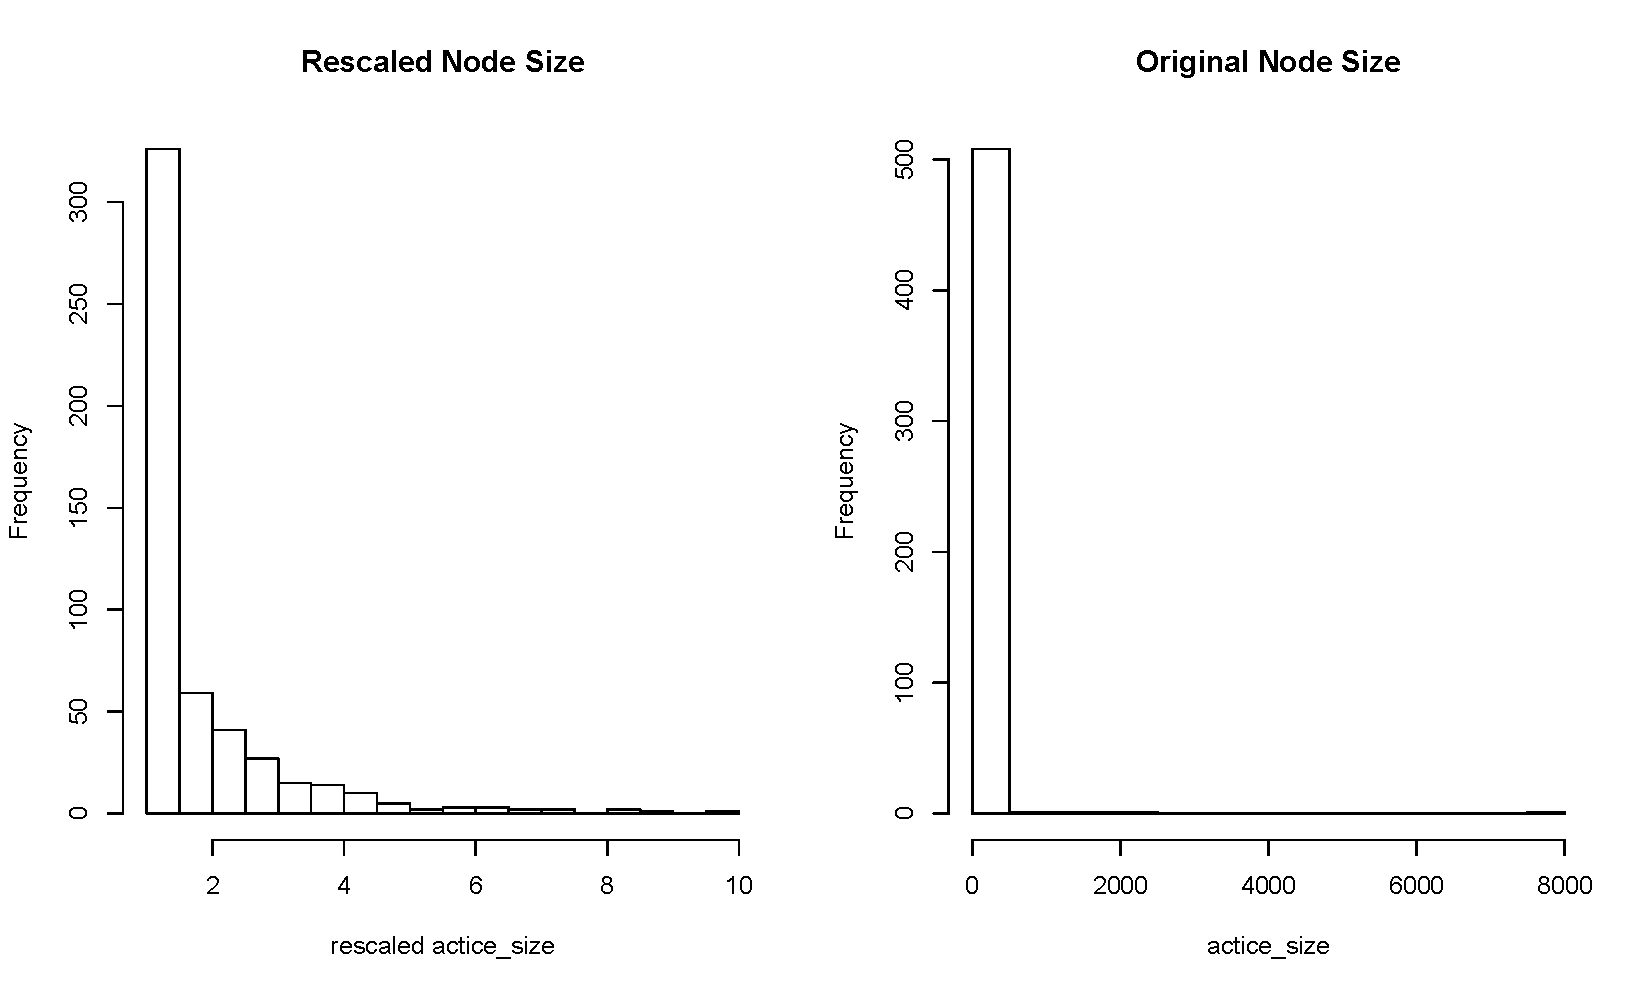
\includegraphics[width=.9\textwidth]{report_rescaled_size}
\end{figure}
\begin{figure}[ht]
\caption{Visualizing Hillary Clinton Received and Sent E-mails}
\label{fig:splitnw}
\centering
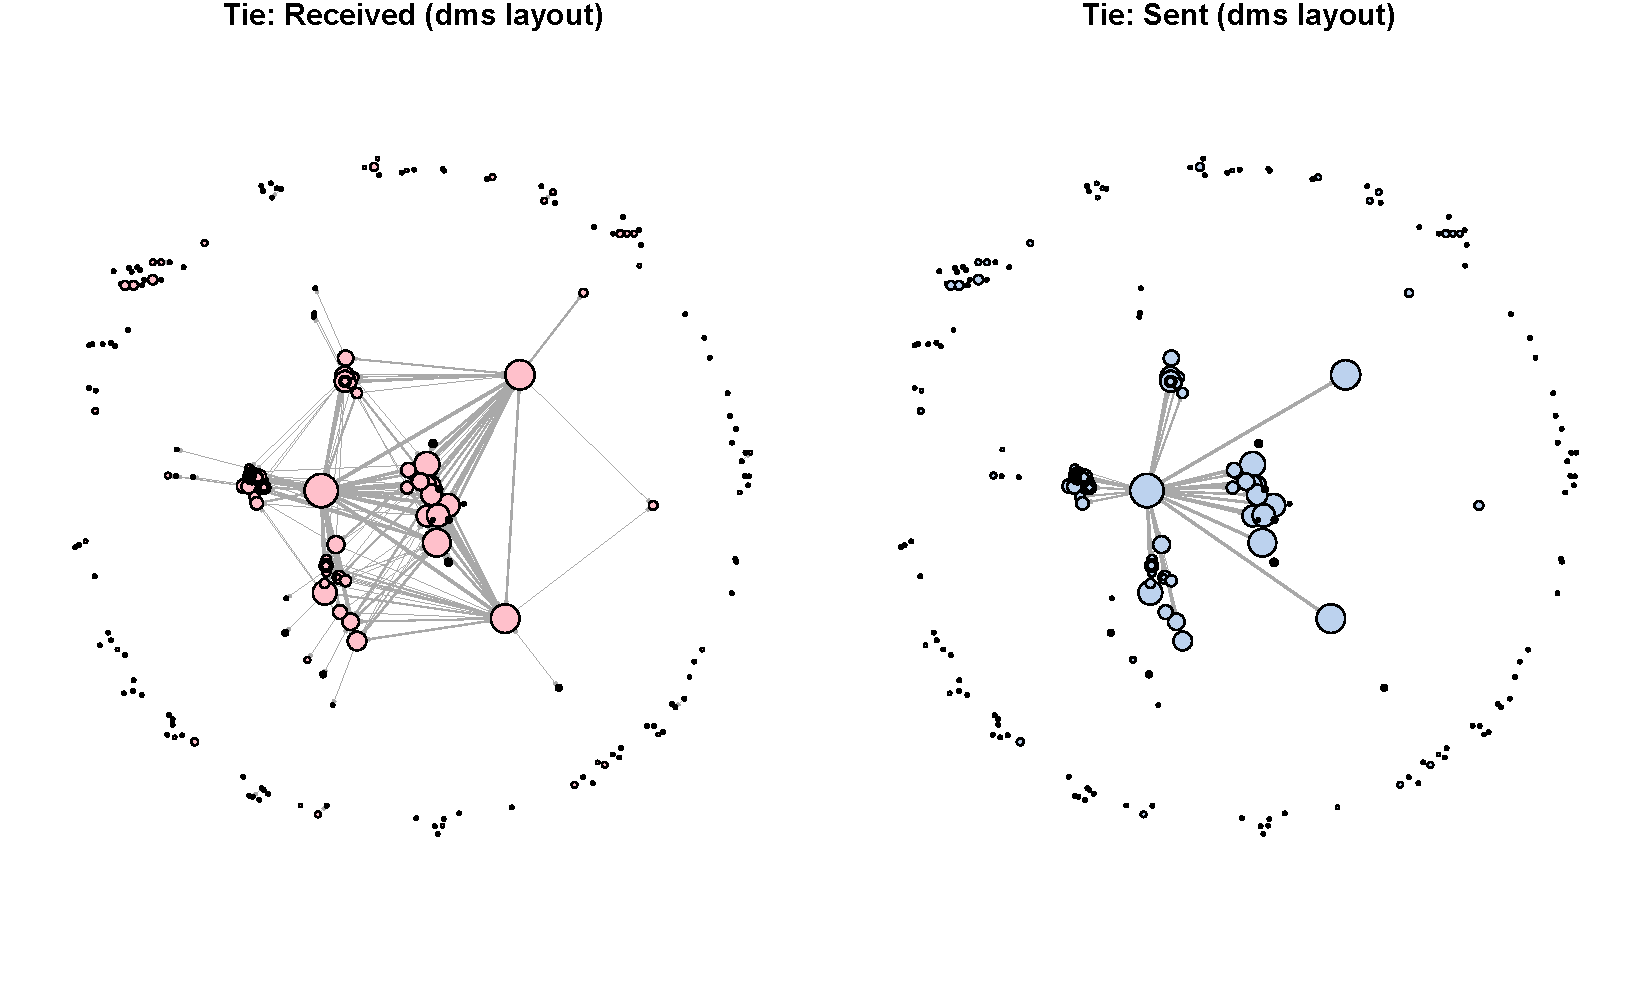
\includegraphics[width=.9\textwidth]{report_network_compare}
\end{figure}

\clearpage
As we have mentioned in Subsection \ref{sna_data}, we can split the network by the edge type.

\subsection{Network Descriptives}
We examine the Hillary Clinton Email network by studying properties of the smaller units - dyads (pairs) and triads (triangles).   

We first calculate the {\bf density} of this network, which gives us an idea about the extent to which the entire network is connected. The density of a directed network is calculated as Equation (\ref{eqt:density}).
\begin{equation}
\label{eqt:density}
\mbox{density }= \frac{\mbox{total number of edges}}{\mbox{number of edges if all nodes were connected}}
\end{equation}
The density of the HC e-mail network is $0.0028<0.01$, which indicates that this network is not at all well-connected. That is, less than $10\%$ of the people within this network are connected. 

A dyad is the smallest possible social group in a network. Such simplistic unit is worth studying in sociology, because two people in a dyad can be linked via some rather exclusive and intimate type of connections, such as ``romantic interetst, family relation,[... ,] partners in crime'' (Wikipedia, Dyad (sociology)\cite{wiki_dyad}.   Among all the $739$ edges in the HC e-mail network, there are $106$ mutual dyads (i.e. double directional links between two individuals), and $527$ asymmetric dyads (the connection only goes one-way). Thus, the proportion of mutual dyads is $\frac{2 \times 106}{739}=0.2869$. This property is called {\bf reciprocity}, which in the context of an e-mail network, gives a rough idea about the dynamic of people's interaction as well as information flow in this network. That is, among all the connected people, about $30\%$ of the information was communicated and exchanged. 

The study of triads is also significant in sociology, as this type of human group is conceptualized to bear more communicational interactions than a dyad. ``For example: adding an extra person, therefore creating a triad, this can result in different language barriers, personal connection, and an overall impression of the third person.'' (Wikipedia, Triad (sociology)\cite{wiki_triad}.Since the goal of our project is to use SNA as a auxiliary  tool to extract important information (both e-mail content and people's association), the study of triads is beyond the scope of our report. However, we do include a brief frequency summary of different forms of triads in our network in the Appendix \ref{App:AppendixB}.
\subsection{Community Detection}
Based on our network, we can use clustering algorithms to find subgroups in the network and thus detect the communities. Because we are analyzing a one-person-centered network, we expect saliently large weight on this person's node and some of the associated edges, which may be coufounding for community detection. And as we are more curious about the unknown in the network, we propose to exclude those HC originated edges from the network. Recall that the sub-networks in Figure \ref{fig:splitnw} - the one for Received e-mails (Left Figure \ref{fig:splitnw}) preserves the structure of the whole network (Figure \ref{fig:improvednw}), while there are less edges coming out of the network center.  

We applied the Fast Greedy Modularity Optimization algorithm (see A Clauset, MEJ Newman and C Moore \cite{greedy_mod} for the details) to the Received E-mails sub-network to find community structure. The algorithm yields a lot of the single-node community and one community of extremely large size - this was all expected as we are dealing with a one-individual centered network. However, we can examine the communities of size $3$ to $10$ and we do obtain some informative communities that can pass on to the later stage of our project. Table \ref{tab:greedy} shows some of the communities we obtain through Modularity Optimization.
\begin{table}
\caption{Communities Detected by Modularity Optimization}
\label{tab:greedy}
\centering
\begin{tabular}{|l |c| l|}\hline
{\bf ID} & \bf Size & \bf Individuals \\ \hline \hline
\bf 11 & $4$ & \verb+"Bill Clinton"   "Chelsea Clinton"  "Tsakina Elbegdori"    "dad mom"+ \\ \hline
\bf 4 & $6$ & \verb+"Betsy Ebeling"    "Bonnie Klehr"     "Doug Hattaway"    "Robert Russo"+\\
&& \verb+"abdinh@state.gov" "bonnie klehr"+\\ \hline
{\bf 5} & $4$ &\verb+"Kris Balderston" "Mark Penn"       "Marty Torrey"    "Michael Fuchs"+\\ \hline
{\bf 3} & $9$ & \verb+"Harold Hongju Koh"    "Jeffrey Feltman"      "Jennifer Robinson"+\\
&& \verb+"Megan Rooney"         "eichensehr kristen e" "hooke kathleen h"+\\
&& \verb+"johnson clifton m"    "townley stephen g"    "jake.sullivan h"+ \\
\hline 
\end{tabular}
\end{table}

From Table \ref{tab:greedy}, we see that with the exception of one individual ``Tsakina Elbegdori'' (the President of Mongolia), people in Community 11 are linked to Hillary Clinton (and each other) via family relation. Community 4 involves people who are related to Hillary Clinton's public relatations and communications strategy matters. For example, Betsy Ebeling is an old and close friend of her, who has played an important role in building a positive public image for HC and antidoting the attacks that Hillary Clinton is untrustworthy. Within the same network, we see Bonnie Ward Klehr (with duplicated labels), who not only is a high school friend of Clinton's, but also designs jewelrys for HC to wear on campaign trail. And we also see people of the similar nature in this community, Doug Hattaway, who was in charge of strategic communications for HC's 2008 presidential campaign, and Robert Russo, Director of Correspondences and Briefings for the Hillary for America campaign this year. 

With these communities we detected in our network, we hope to gain deeper understanding of Hillary Clinton's e-mails from a social interaction perspective and also help us efficiently browse this large corpus of documents/e-mails to extract as much important information as possible. 
\clearpage
\appendix
\section{R Commands} \label{App:AppendixA}
\clearpage
\section{Supplement Graphs and Tables} \label{App:AppendixB}
\begin{figure}[ht]
\centering
\caption{Exploring different network layouts}
\label{fig:trylayout}
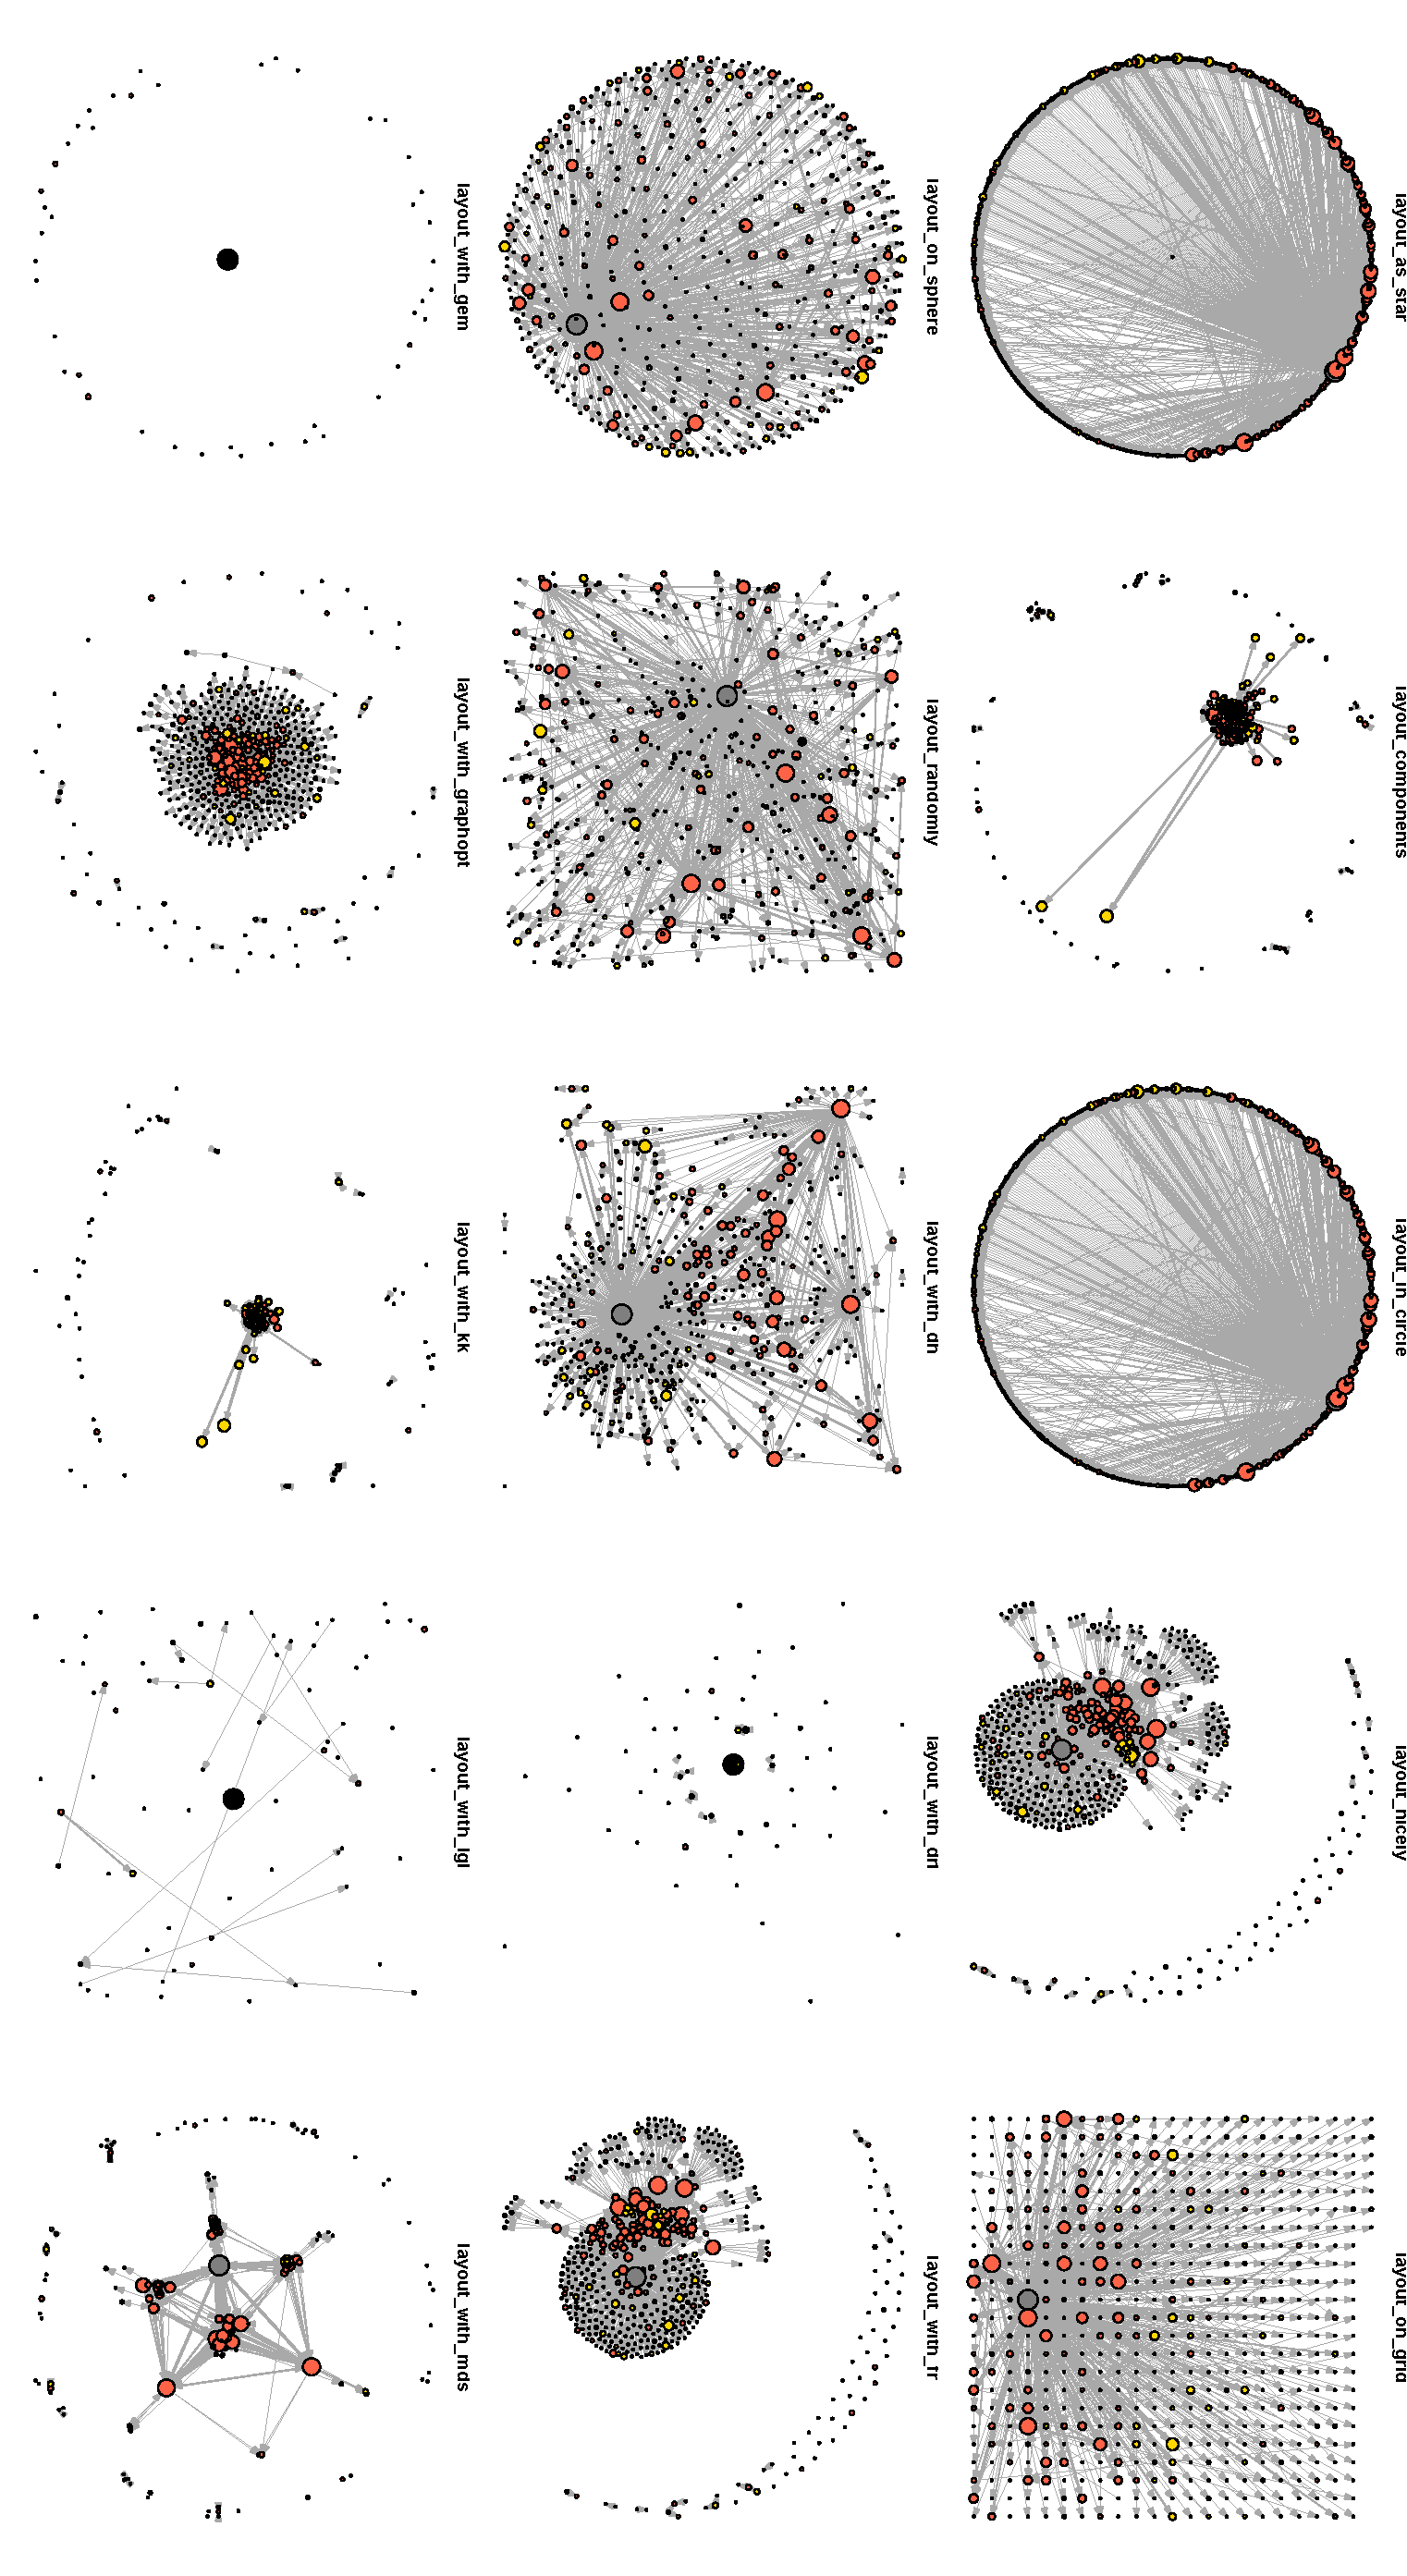
\includegraphics[width=.5\textwidth]{report_explore_layout}
\end{figure}
\clearpage
\begin{thebibliography}{1}
\bibitem{wiki_sna} \verb+https://en.wikipedia.org/wiki/Social_network_analysis+
\bibitem{wiki_dyad} \verb+https://en.wikipedia.org/wiki/Dyad_(sociology)+
\bibitem{wiki_triad} \verb+https://en.wikipedia.org/wiki/Triad_(sociology)+
\bibitem{greedy_mod} A Clauset, MEJ Newman, C Moore: Finding community structure in very large networks, \verb+http://www.arxiv.org/abs/cond-mat/0408187+ .
\end{thebibliography}
\end{document}